% Options for packages loaded elsewhere
\PassOptionsToPackage{unicode}{hyperref}
\PassOptionsToPackage{hyphens}{url}
%
\documentclass[
  man,floatsintext]{apa6}
\usepackage{amsmath,amssymb}
\usepackage{iftex}
\ifPDFTeX
  \usepackage[T1]{fontenc}
  \usepackage[utf8]{inputenc}
  \usepackage{textcomp} % provide euro and other symbols
\else % if luatex or xetex
  \usepackage{unicode-math} % this also loads fontspec
  \defaultfontfeatures{Scale=MatchLowercase}
  \defaultfontfeatures[\rmfamily]{Ligatures=TeX,Scale=1}
\fi
\usepackage{lmodern}
\ifPDFTeX\else
  % xetex/luatex font selection
\fi
% Use upquote if available, for straight quotes in verbatim environments
\IfFileExists{upquote.sty}{\usepackage{upquote}}{}
\IfFileExists{microtype.sty}{% use microtype if available
  \usepackage[]{microtype}
  \UseMicrotypeSet[protrusion]{basicmath} % disable protrusion for tt fonts
}{}
\makeatletter
\@ifundefined{KOMAClassName}{% if non-KOMA class
  \IfFileExists{parskip.sty}{%
    \usepackage{parskip}
  }{% else
    \setlength{\parindent}{0pt}
    \setlength{\parskip}{6pt plus 2pt minus 1pt}}
}{% if KOMA class
  \KOMAoptions{parskip=half}}
\makeatother
\usepackage{xcolor}
\usepackage{color}
\usepackage{fancyvrb}
\newcommand{\VerbBar}{|}
\newcommand{\VERB}{\Verb[commandchars=\\\{\}]}
\DefineVerbatimEnvironment{Highlighting}{Verbatim}{commandchars=\\\{\}}
% Add ',fontsize=\small' for more characters per line
\usepackage{framed}
\definecolor{shadecolor}{RGB}{248,248,248}
\newenvironment{Shaded}{\begin{snugshade}}{\end{snugshade}}
\newcommand{\AlertTok}[1]{\textcolor[rgb]{0.94,0.16,0.16}{#1}}
\newcommand{\AnnotationTok}[1]{\textcolor[rgb]{0.56,0.35,0.01}{\textbf{\textit{#1}}}}
\newcommand{\AttributeTok}[1]{\textcolor[rgb]{0.13,0.29,0.53}{#1}}
\newcommand{\BaseNTok}[1]{\textcolor[rgb]{0.00,0.00,0.81}{#1}}
\newcommand{\BuiltInTok}[1]{#1}
\newcommand{\CharTok}[1]{\textcolor[rgb]{0.31,0.60,0.02}{#1}}
\newcommand{\CommentTok}[1]{\textcolor[rgb]{0.56,0.35,0.01}{\textit{#1}}}
\newcommand{\CommentVarTok}[1]{\textcolor[rgb]{0.56,0.35,0.01}{\textbf{\textit{#1}}}}
\newcommand{\ConstantTok}[1]{\textcolor[rgb]{0.56,0.35,0.01}{#1}}
\newcommand{\ControlFlowTok}[1]{\textcolor[rgb]{0.13,0.29,0.53}{\textbf{#1}}}
\newcommand{\DataTypeTok}[1]{\textcolor[rgb]{0.13,0.29,0.53}{#1}}
\newcommand{\DecValTok}[1]{\textcolor[rgb]{0.00,0.00,0.81}{#1}}
\newcommand{\DocumentationTok}[1]{\textcolor[rgb]{0.56,0.35,0.01}{\textbf{\textit{#1}}}}
\newcommand{\ErrorTok}[1]{\textcolor[rgb]{0.64,0.00,0.00}{\textbf{#1}}}
\newcommand{\ExtensionTok}[1]{#1}
\newcommand{\FloatTok}[1]{\textcolor[rgb]{0.00,0.00,0.81}{#1}}
\newcommand{\FunctionTok}[1]{\textcolor[rgb]{0.13,0.29,0.53}{\textbf{#1}}}
\newcommand{\ImportTok}[1]{#1}
\newcommand{\InformationTok}[1]{\textcolor[rgb]{0.56,0.35,0.01}{\textbf{\textit{#1}}}}
\newcommand{\KeywordTok}[1]{\textcolor[rgb]{0.13,0.29,0.53}{\textbf{#1}}}
\newcommand{\NormalTok}[1]{#1}
\newcommand{\OperatorTok}[1]{\textcolor[rgb]{0.81,0.36,0.00}{\textbf{#1}}}
\newcommand{\OtherTok}[1]{\textcolor[rgb]{0.56,0.35,0.01}{#1}}
\newcommand{\PreprocessorTok}[1]{\textcolor[rgb]{0.56,0.35,0.01}{\textit{#1}}}
\newcommand{\RegionMarkerTok}[1]{#1}
\newcommand{\SpecialCharTok}[1]{\textcolor[rgb]{0.81,0.36,0.00}{\textbf{#1}}}
\newcommand{\SpecialStringTok}[1]{\textcolor[rgb]{0.31,0.60,0.02}{#1}}
\newcommand{\StringTok}[1]{\textcolor[rgb]{0.31,0.60,0.02}{#1}}
\newcommand{\VariableTok}[1]{\textcolor[rgb]{0.00,0.00,0.00}{#1}}
\newcommand{\VerbatimStringTok}[1]{\textcolor[rgb]{0.31,0.60,0.02}{#1}}
\newcommand{\WarningTok}[1]{\textcolor[rgb]{0.56,0.35,0.01}{\textbf{\textit{#1}}}}
\usepackage{graphicx}
\makeatletter
\def\maxwidth{\ifdim\Gin@nat@width>\linewidth\linewidth\else\Gin@nat@width\fi}
\def\maxheight{\ifdim\Gin@nat@height>\textheight\textheight\else\Gin@nat@height\fi}
\makeatother
% Scale images if necessary, so that they will not overflow the page
% margins by default, and it is still possible to overwrite the defaults
% using explicit options in \includegraphics[width, height, ...]{}
\setkeys{Gin}{width=\maxwidth,height=\maxheight,keepaspectratio}
% Set default figure placement to htbp
\makeatletter
\def\fps@figure{htbp}
\makeatother
\setlength{\emergencystretch}{3em} % prevent overfull lines
\providecommand{\tightlist}{%
  \setlength{\itemsep}{0pt}\setlength{\parskip}{0pt}}
\setcounter{secnumdepth}{-\maxdimen} % remove section numbering
% Make \paragraph and \subparagraph free-standing
\ifx\paragraph\undefined\else
  \let\oldparagraph\paragraph
  \renewcommand{\paragraph}[1]{\oldparagraph{#1}\mbox{}}
\fi
\ifx\subparagraph\undefined\else
  \let\oldsubparagraph\subparagraph
  \renewcommand{\subparagraph}[1]{\oldsubparagraph{#1}\mbox{}}
\fi
% definitions for citeproc citations
\NewDocumentCommand\citeproctext{}{}
\NewDocumentCommand\citeproc{mm}{%
  \begingroup\def\citeproctext{#2}\cite{#1}\endgroup}
\makeatletter
 % allow citations to break across lines
 \let\@cite@ofmt\@firstofone
 % avoid brackets around text for \cite:
 \def\@biblabel#1{}
 \def\@cite#1#2{{#1\if@tempswa , #2\fi}}
\makeatother
\newlength{\cslhangindent}
\setlength{\cslhangindent}{1.5em}
\newlength{\csllabelwidth}
\setlength{\csllabelwidth}{3em}
\newenvironment{CSLReferences}[2] % #1 hanging-indent, #2 entry-spacing
 {\begin{list}{}{%
  \setlength{\itemindent}{0pt}
  \setlength{\leftmargin}{0pt}
  \setlength{\parsep}{0pt}
  % turn on hanging indent if param 1 is 1
  \ifodd #1
   \setlength{\leftmargin}{\cslhangindent}
   \setlength{\itemindent}{-1\cslhangindent}
  \fi
  % set entry spacing
  \setlength{\itemsep}{#2\baselineskip}}}
 {\end{list}}
\usepackage{calc}
\newcommand{\CSLBlock}[1]{\hfill\break\parbox[t]{\linewidth}{\strut\ignorespaces#1\strut}}
\newcommand{\CSLLeftMargin}[1]{\parbox[t]{\csllabelwidth}{\strut#1\strut}}
\newcommand{\CSLRightInline}[1]{\parbox[t]{\linewidth - \csllabelwidth}{\strut#1\strut}}
\newcommand{\CSLIndent}[1]{\hspace{\cslhangindent}#1}
\ifLuaTeX
\usepackage[bidi=basic]{babel}
\else
\usepackage[bidi=default]{babel}
\fi
\babelprovide[main,import]{english}
% get rid of language-specific shorthands (see #6817):
\let\LanguageShortHands\languageshorthands
\def\languageshorthands#1{}
% Manuscript styling
\usepackage{upgreek}
\captionsetup{font=singlespacing,justification=justified}

% Table formatting
\usepackage{longtable}
\usepackage{lscape}
% \usepackage[counterclockwise]{rotating}   % Landscape page setup for large tables
\usepackage{multirow}		% Table styling
\usepackage{tabularx}		% Control Column width
\usepackage[flushleft]{threeparttable}	% Allows for three part tables with a specified notes section
\usepackage{threeparttablex}            % Lets threeparttable work with longtable

% Create new environments so endfloat can handle them
% \newenvironment{ltable}
%   {\begin{landscape}\centering\begin{threeparttable}}
%   {\end{threeparttable}\end{landscape}}
\newenvironment{lltable}{\begin{landscape}\centering\begin{ThreePartTable}}{\end{ThreePartTable}\end{landscape}}

% Enables adjusting longtable caption width to table width
% Solution found at http://golatex.de/longtable-mit-caption-so-breit-wie-die-tabelle-t15767.html
\makeatletter
\newcommand\LastLTentrywidth{1em}
\newlength\longtablewidth
\setlength{\longtablewidth}{1in}
\newcommand{\getlongtablewidth}{\begingroup \ifcsname LT@\roman{LT@tables}\endcsname \global\longtablewidth=0pt \renewcommand{\LT@entry}[2]{\global\advance\longtablewidth by ##2\relax\gdef\LastLTentrywidth{##2}}\@nameuse{LT@\roman{LT@tables}} \fi \endgroup}

% \setlength{\parindent}{0.5in}
% \setlength{\parskip}{0pt plus 0pt minus 0pt}

% Overwrite redefinition of paragraph and subparagraph by the default LaTeX template
% See https://github.com/crsh/papaja/issues/292
\makeatletter
\renewcommand{\paragraph}{\@startsection{paragraph}{4}{\parindent}%
  {0\baselineskip \@plus 0.2ex \@minus 0.2ex}%
  {-1em}%
  {\normalfont\normalsize\bfseries\itshape\typesectitle}}

\renewcommand{\subparagraph}[1]{\@startsection{subparagraph}{5}{1em}%
  {0\baselineskip \@plus 0.2ex \@minus 0.2ex}%
  {-\z@\relax}%
  {\normalfont\normalsize\itshape\hspace{\parindent}{#1}\textit{\addperi}}{\relax}}
\makeatother

\makeatletter
\usepackage{etoolbox}
\patchcmd{\maketitle}
  {\section{\normalfont\normalsize\abstractname}}
  {\section*{\normalfont\normalsize\abstractname}}
  {}{\typeout{Failed to patch abstract.}}
\patchcmd{\maketitle}
  {\section{\protect\normalfont{\@title}}}
  {\section*{\protect\normalfont{\@title}}}
  {}{\typeout{Failed to patch title.}}
\makeatother

\usepackage{xpatch}
\makeatletter
\xapptocmd\appendix
  {\xapptocmd\section
    {\addcontentsline{toc}{section}{\appendixname\ifoneappendix\else~\theappendix\fi\\: #1}}
    {}{\InnerPatchFailed}%
  }
{}{\PatchFailed}
\keywords{response times, event history analysis, Bayesian regression models\newline\indent Word count: X}
\usepackage{lineno}

\linenumbers
\usepackage{csquotes}
\raggedbottom
\ifLuaTeX
  \usepackage{selnolig}  % disable illegal ligatures
\fi
\usepackage{bookmark}
\IfFileExists{xurl.sty}{\usepackage{xurl}}{} % add URL line breaks if available
\urlstyle{same}
\hypersetup{
  pdftitle={A tutorial on Bayesian and Frequentist Event History Analysis for psychological time-to-event data},
  pdfauthor={Sven Panis1 \& Richard Ramsey1},
  pdflang={en-EN},
  pdfkeywords={response times, event history analysis, Bayesian regression models},
  hidelinks,
  pdfcreator={LaTeX via pandoc}}

\title{A tutorial on Bayesian and Frequentist Event History Analysis for psychological time-to-event data}
\author{Sven Panis\textsuperscript{1} \& Richard Ramsey\textsuperscript{1}}
\date{}


\shorttitle{Tutorial on hazard modeling}

\authornote{

Neural Control of Movement lab, Department of Health Sciences and Technology (D-HEST).

The authors made the following contributions. Sven Panis: Conceptualization, Writing - Original Draft Preparation, Writing - Review \& Editing; Richard Ramsey: Conceptualization, Writing - Review \& Editing, Supervision.

Correspondence concerning this article should be addressed to Sven Panis, ETH GLC, room G16.2, Gloriastrasse 37/39, 8006 Zürich. E-mail: \href{mailto:sven.panis@hest.ethz.ch}{\nolinkurl{sven.panis@hest.ethz.ch}}

}

\affiliation{\vspace{0.5cm}\textsuperscript{1} ETH Zürich}

\abstract{%
Time-to-event data such as response times, saccade latencies, and fixation durations are ubiquitous in experimental psychology. To move beyond mean performance measures, various distributional analyses have been proposed. Here we focus on one particular distributional analysis known as discrete-time event history analysis, a.k.a. hazard analysis, duration analysis, failure-time analysis, survival analysis, and transition analysis. Across four tutorials that we make publicly available on Github and OSF, we illustrate how to calculate and interpret descriptive statistics, and how to implement Bayesian and frequentist regression models, using the R packages tidyverse, brms, and lme4. We discuss how to manage inter-individual differences, implications for experimental design, and how to select among various options when analysing time-to-event data using discrete-time survival analysis.
}



\begin{document}
\maketitle

\section{Introduction}\label{introduction}

In experimental psychology, it is still standard practice to analyse response times (RTs), saccade latencies, and fixation durations using analysis-of-variance. However, differences in means conceal when an experimental effect starts, how long it lasts, and whether its onset is time-locked to other events. Such information is useful not only for interpretation, but also for cognitive psychophysiology and computational model selection (Panis, Schmidt, Wolkersdorfer, \& Schmidt, 2020).
In this tutorial we focus on a distributional method for analyzing time-to-event data that is known as discrete-time event history analysis (EHA), a.k.a. survival, hazard, duration, failure-time, and transition analysis (Allison, 1982, 2010; Singer \& Willett, 2003). Across four tutorials that we make publicly available on Github and OSF, we illustrate how to calculate and interpret descriptive statistics, and how to implement Bayesian and frequentist regression models, using the R packages tidyverse, brms, and lme4.

To apply EHA, one must be able to define the event of interest (any qualitative change that can be situated in time, e.g., a button press, saccade onset, fixation offset), time point zero (e.g., target stimulus onset, fixation onset), and measure the passage of time between time point zero and event occurrence in discrete or continuous time units.

The shape of a distribution of waiting times can be described in multiple ways (Luce, 1991). Let RT be a continous random variable denoting a particular person's response time in a particular experimental condition. Because waiting times can only increase, continuous-time EHA does not focus on the cumulative distribution function F(t) = P(RT \(\leq\) t) and its derivative, the probability density function f(t) = F(t)', but on the survivor function S(t) = P(RT \(>\) t) and the hazard rate function \(\lambda\)(t) = f(t)/S(t). The hazard rate function gives you the instantaneous rate of event occurrence at time point t, given that the event has not occurred yet.

Similarly, after dividing time in discrete, contiguous time bins indexed by t, let RT be a discrete random variable denoting the rank of the time bin in which a particular person's response occurs in a particular experimental condition. Discrete-time EHA focuses on the discrete-time survivor function S(t) = P(RT \(>\) t) and the discrete-time hazard function h(t) = P(RT = t\textbar{} RT \(\geq\) t), and not on the probability mass function and the cumulative distribution function. The discrete-time hazard probability function gives you the probability that the event occurs (sometime) in bin t, given that the event has not occurred yet in previous bins. For two-choice RT data, the discrete-time hazard function can be extended with the conditional accuracy function ca(t) = P(correct \textbar{} RT = t), which gives you the probability that a response is correct given that it has been emitted in time bin t (Allison, 2010; Kantowitz \& Pachella, 2021; Wickelgren, 1977). This latter function is also known as the micro-level speed-accuracy tradeoff function.

Statisticians and mathematical psychologists recommend focusing on the hazard function when analyzing time-to-event data for various reasons. First, as discussed by Holden, Van Orden, and Turvey (2009), ``probability density functions can appear nearly identical, both statistically and to the naked eye, and yet are clearly different on the basis of their hazard functions (but not vice versa). Hazard functions are thus more diagnostic than density functions'' (p.~331).
Second, because RT distributions may differ from one another in multiple ways, Townsend (1990) developed a dominance hierarchy of statistical differences between two arbitrary distributions A and B. For example, if F\textsubscript{A}(t) \textgreater{} F\textsubscript{B}(t) for all t, then both cumulative distribution functions are said to show a complete ordering. Townsend (1990) showed that a complete ordering on the hazard functions ---\(\lambda\)\textsubscript{A}(t) \textgreater{} \(\lambda\)\textsubscript{B}(t) for all t--- implies a complete ordering on both the cumulative distribution and survivor functions ---F\textsubscript{A}(t) \textgreater{} F\textsubscript{B}(t) and S\textsubscript{A}(t) \textless{} S\textsubscript{B}(t)--- which in turn implies an ordering on the mean latencies ---mean A \textless{} mean B. In contrast, an ordering on two means does not imply a complete ordering on the corresponding F(t) and S(t) functions, and a complete ordering on these latter functions does not imply a complete ordering on the corresponding hazard functions. This means that stronger conclusions can be drawn from data when comparing the hazard functions using EHA. For example, when mean A \textless{} mean B, the hazard functions might show a complete ordering (i.e., for all t), a partial ordering (e.g., only for t \textgreater{} 300 ms, or only for t \textless{} 500 ms), or they may cross each other one or more times.
Third, EHA does not discard right-censored observations when estimating hazard functions, that is, trials for which we do not observe a response during the data collection period so that we only know that the RT must be larger than some value. This is important because although a few right-censored observations are inevitable in most RT tasks, a lot of right-censored observations are expected in experiments on masking, the attentional blink, and so forth.
Fourth, hazard modeling allows incorporating time-varying explanatory covariates such as heart rate, electroencephalogram (EEG) signal amplitude, gaze location, etc. (Allison, 2010) which is useful for cognitive psychophysiology (Meyer, Osman, Irwin, \& Yantis, 1988).
Finally, as explained by Kelso, Dumas, and Tognoli (2013), it is crucial to first have a precise description of the macroscopic behavior of a system (here: h(t) and ca(t) functions) in order to know what to derive on the microscopic level. For example, fitting parametric functions or computational models to data without studying the shape of the h(t) and ca(t) functions can miss important features in the data (Panis, Moran, Wolkersdorfer, \& Schmidt, 2020; Panis \& Schmidt, 2016).

We focus on factorial within-subject designs in which a large number of observations are made on a relatively small number of participants (small-\emph{N} designs). This approach emphasizes the precision and reproducibility of data patterns at the individual participant level to increase the inferential validity of the design (Baker et al., 2021; Smith \& Little, 2018). In contrast to the large-\emph{N} design that averages across many participants without being able to scrutinize individual data patterns, small-\emph{N} designs retain crucial information about the data patterns of individual observers. This is of great advantage whenever participants differ systematically in their strategies or in the time-courses of their effects, so that blindly averaging them would lead to misleading data patterns. Indeed, Smith and Little (2018) argue that, ``if psychology is to be a mature quantitative science, then its primary theoretical aim should be to investigate systematic functional relationships as they are manifested at the individual participant level'' (p.~2083). Note that because statistical power derives both from the number of participants and from the number of repeated measures per participant and condition, small-\emph{N} designs can have excellent power (Baker et al., 2021; Smith \& Little, 2018).

We used R (Version 4.4.0; R Core Team, 2024)\footnote{We, furthermore, used the R-packages \emph{citr} (Version 0.3.2; Aust, 2019), \emph{dplyr} (Version 1.1.4; Wickham, François, Henry, Müller, \& Vaughan, 2023), \emph{forcats} (Version 1.0.0; Wickham, 2023a), \emph{ggplot2} (Version 3.5.1; Wickham, 2016), \emph{lubridate} (Version 1.9.3; Grolemund \& Wickham, 2011), \emph{papaja} (Version 0.1.2.9000; Aust \& Barth, 2023), \emph{patchwork} (Version 1.2.0; Pedersen, 2024), \emph{purrr} (Version 1.0.2; Wickham \& Henry, 2023), \emph{RColorBrewer} (Version 1.1.3; Neuwirth, 2022), \emph{readr} (Version 2.1.5; Wickham, Hester, \& Bryan, 2024), \emph{stringr} (Version 1.5.1; Wickham, 2023b), \emph{tibble} (Version 3.2.1; Müller \& Wickham, 2023), \emph{tidyr} (Version 1.3.1; Wickham, Vaughan, \& Girlich, 2024), \emph{tidyverse} (Version 2.0.0; Wickham et al., 2019), and \emph{tinylabels} (Version 0.2.4; Barth, 2023).} for all reported analyses. Web links are printed in bold.

\section{Tutorial 1: Calculating descriptive statistics using a life table}\label{tutorial-1-calculating-descriptive-statistics-using-a-life-table}

To illustrate how to quickly set up life tables for calculating the descriptive statistics (functions of discrete time), we use a published data set on masked response priming from Panis and Schmidt (2016), available on \href{https://www.researchgate.net/publication/304069212_What_Is_Shaping_RT_and_Accuracy_Distributions_Active_and_Selective_Response_Inhibition_Causes_the_Negative_Compatibility_Effect}{\textbf{ResearchGate}}.
In their first experiment, Panis and Schmidt (2016) presented a double arrow for 94 ms that pointed left or right as the target stimulus with an onset at time point zero in each trial. Participants had to indicate the direction in which the double arrow pointed using their corresponding index finger, within 800 ms after target onset. Response time and accuracy were recorded on each trial. Prime type (blank, congruent, incongruent) and mask type were manipulated. Here we focus on the subset of trials in which no mask was presented. The 13-ms prime stimulus was a double arrow with onset at -187 ms for the congruent (same direction as target) and incongruent (opposite direction as target) prime conditions.

After loading in the data file, one has to (a) supply required column names, and (b) specify the factor condition with the correct levels and labels.
The required column names are as follows:

\begin{itemize}
\tightlist
\item
  ``pid'', indicating unique participant IDs;
\item
  ``trial'', indicating each unique trial per participant;
\item
  ``condition'', a factor indicating the levels of the independent variable (1, 2, \ldots) and the corresponding labels;
\item
  ``rt'', indicating the response times in ms;
\item
  ``acc'', inicating the accuracies (1/0).
\end{itemize}

In the code of Tutorial 1, this is accomplished as follows.

\scriptsize

\begin{Shaded}
\begin{Highlighting}[]
\NormalTok{data\_wr }\OtherTok{\textless{}{-}} \FunctionTok{read\_csv}\NormalTok{(}\StringTok{"../Tutorial\_1\_descriptive\_stats/data/DataExp1\_6subjects\_wrangled.csv"}\NormalTok{)}
\FunctionTok{colnames}\NormalTok{(data\_wr) }\OtherTok{\textless{}{-}} \FunctionTok{c}\NormalTok{(}\StringTok{"pid"}\NormalTok{,}\StringTok{"bl"}\NormalTok{,}\StringTok{"tr"}\NormalTok{,}\StringTok{"condition"}\NormalTok{,}\StringTok{"resp"}\NormalTok{,}\StringTok{"acc"}\NormalTok{,}\StringTok{"rt"}\NormalTok{,}\StringTok{"trial"}\NormalTok{) }
\NormalTok{data\_wr }\OtherTok{\textless{}{-}}\NormalTok{ data\_wr }\SpecialCharTok{\%\textgreater{}\%} 
  \FunctionTok{mutate}\NormalTok{(}\AttributeTok{condition =}\NormalTok{ condition }\SpecialCharTok{+} \DecValTok{1}\NormalTok{, }\CommentTok{\# original levels were 0, 1, 2.}
         \AttributeTok{condition =} \FunctionTok{factor}\NormalTok{(condition, }\AttributeTok{levels=}\FunctionTok{c}\NormalTok{(}\DecValTok{1}\NormalTok{,}\DecValTok{2}\NormalTok{,}\DecValTok{3}\NormalTok{), }\AttributeTok{labels=}\FunctionTok{c}\NormalTok{(}\StringTok{"blank"}\NormalTok{,}\StringTok{"congruent"}\NormalTok{,}\StringTok{"incongruent"}\NormalTok{)))}
\end{Highlighting}
\end{Shaded}

\normalsize

To set up the life tables and plots of the discrete-time functions h(t), S(t) and ca(t) using functional programming, one has to nest the data within participants using the group\_nest() function, and supply a user-defined censoring time and bin width to our function ``censor()'', as follows.

\scriptsize

\begin{Shaded}
\begin{Highlighting}[]
\NormalTok{data\_nested }\OtherTok{\textless{}{-}}\NormalTok{ data\_wr }\SpecialCharTok{\%\textgreater{}\%} \FunctionTok{group\_nest}\NormalTok{(pid)}
\NormalTok{data\_final }\OtherTok{\textless{}{-}}\NormalTok{ data\_nested }\SpecialCharTok{\%\textgreater{}\%} 
  \FunctionTok{mutate}\NormalTok{(}\AttributeTok{censored  =} \FunctionTok{map}\NormalTok{(data, censor, }\DecValTok{600}\NormalTok{, }\DecValTok{40}\NormalTok{)) }\SpecialCharTok{\%\textgreater{}\%}   \CommentTok{\# ! user input: censoring time, and bin width}
  \FunctionTok{mutate}\NormalTok{(}\AttributeTok{ptb\_data  =} \FunctionTok{map}\NormalTok{(censored, ptb)) }\SpecialCharTok{\%\textgreater{}\%}           \CommentTok{\# create person{-}trial{-}bin dataset}
  \FunctionTok{mutate}\NormalTok{(}\AttributeTok{lifetable =} \FunctionTok{map}\NormalTok{(ptb\_data, setup\_lt)) }\SpecialCharTok{\%\textgreater{}\%}      \CommentTok{\# create life tables without ca(t)}
  \FunctionTok{mutate}\NormalTok{(}\AttributeTok{condacc   =} \FunctionTok{map}\NormalTok{(censored, calc\_ca)) }\SpecialCharTok{\%\textgreater{}\%}       \CommentTok{\# calculate ca(t)}
  \FunctionTok{mutate}\NormalTok{(}\AttributeTok{lifetable\_ca =} \FunctionTok{map2}\NormalTok{(lifetable, condacc, join\_lt\_ca)) }\SpecialCharTok{\%\textgreater{}\%}    \CommentTok{\# create life tables with ca(t)}
  \FunctionTok{mutate}\NormalTok{(}\AttributeTok{plot      =} \FunctionTok{map2}\NormalTok{(}\AttributeTok{.x =}\NormalTok{ lifetable\_ca, }\AttributeTok{.y =}\NormalTok{ pid, plot\_eha,}\DecValTok{1}\NormalTok{))  }\CommentTok{\# create plots }
\end{Highlighting}
\end{Shaded}

\normalsize

Note that the censoring time should be a multiple of the bin width (both in ms). The censoring time should be a time point after which no informative responses are expected anymore. In experiments that implement a response deadline in each trial the censoring time can equal that deadline time point. Trials with a RT larger than the censoring time, or trials in which no response is emitted during the data collection period, are treated as right-censored observations in EHA. In other words, these trials are not discarded, because they contain the information that the event did not occur before the censoring time. Removing such trials before calculating the mean event time can introduce a sampling bias. The person-trial-bin oriented dataset has one row for each time bin of each trial that is at risk for event occurrence. The variable ``event'' in the person-trial-bin oriented data set indicates whether a response occurs (1) or not (0) for each bin.
One can now inspect different aspects, including the life table for a particular condition of a particular subject, and a plot of the different functions for a particular participant.

Table 1 shows the life table for condition ``blank'' (no prime stimulus presented) - compare to Figure 1. A life table includes for each time bin, the risk set (number of trials that are event-free at the start of the bin), the number of observed events, and the estimates of h(t), S(t), ca(t) and their estimated standard errors (se). At time point zero, no events can occur and therefore h(t) and ca(t) are undefined.

Figure 1 displays the discrete-time hazard, survivor, and conditional accuracy functions for each prime condition for participant 6. By using discrete-time h(t) functions of event occurrence - in combination with ca(t) functions for two-choice tasks - one can provide an unbiased, time-varying, and probabilistic description of the latency and accuracy of responses based on all trials of any data set.

For example, for participant 6, the estimated hazard values in bin (240,280{]} are 0.03, 0.17, and 0.22 for the blank, congruent, and incongruent prime conditions, respectively. In other words, when the waiting time has increased until \emph{240 ms} after target onset, then the conditional probability of response occurrence in the next 40 ms is more than five times larger for both prime-present conditions, compared to the blank prime condition.





\begin{table}[H]

\begin{center}
\begin{threeparttable}

\caption{\label{tab:life-table}This is the life table for condition blank of participant 6.}

\begin{tabular}{lllllllll}
\toprule
bin & \multicolumn{1}{c}{risk\_set} & \multicolumn{1}{c}{events} & \multicolumn{1}{c}{hazard} & \multicolumn{1}{c}{se\_haz} & \multicolumn{1}{c}{survival} & \multicolumn{1}{c}{se\_surv} & \multicolumn{1}{c}{ca} & \multicolumn{1}{c}{se\_ca}\\
\midrule
0.00 & 219.00 & NA & NA & NA & 1.00 & 0.00 & NA & NA\\
40.00 & 219.00 & 0.00 & 0.00 & 0.00 & 1.00 & 0.00 & NA & NA\\
80.00 & 219.00 & 0.00 & 0.00 & 0.00 & 1.00 & 0.00 & NA & NA\\
120.00 & 219.00 & 0.00 & 0.00 & 0.00 & 1.00 & 0.00 & NA & NA\\
160.00 & 219.00 & 0.00 & 0.00 & 0.00 & 1.00 & 0.00 & NA & NA\\
200.00 & 219.00 & 0.00 & 0.00 & 0.00 & 1.00 & 0.00 & NA & NA\\
240.00 & 219.00 & 0.00 & 0.00 & 0.00 & 1.00 & 0.00 & NA & NA\\
280.00 & 219.00 & 7.00 & 0.03 & 0.01 & 0.97 & 0.01 & 0.29 & 0.17\\
320.00 & 212.00 & 13.00 & 0.06 & 0.02 & 0.91 & 0.02 & 0.77 & 0.12\\
360.00 & 199.00 & 26.00 & 0.13 & 0.02 & 0.79 & 0.03 & 0.92 & 0.05\\
400.00 & 173.00 & 40.00 & 0.23 & 0.03 & 0.61 & 0.03 & 1.00 & 0.00\\
440.00 & 133.00 & 48.00 & 0.36 & 0.04 & 0.39 & 0.03 & 0.98 & 0.02\\
480.00 & 85.00 & 37.00 & 0.44 & 0.05 & 0.22 & 0.03 & 1.00 & 0.00\\
520.00 & 48.00 & 32.00 & 0.67 & 0.07 & 0.07 & 0.02 & 1.00 & 0.00\\
560.00 & 16.00 & 9.00 & 0.56 & 0.12 & 0.03 & 0.01 & 1.00 & 0.00\\
600.00 & 7.00 & 4.00 & 0.57 & 0.19 & 0.01 & 0.01 & 1.00 & 0.00\\
\bottomrule
\addlinespace
\end{tabular}

\begin{tablenotes}[para]
\normalsize{\textit{Note.} The column named ``bin'' indicates the endpoint of each time bin (in ms), and includes time point zero. se = standard error. ca = conditional accuracy.}
\end{tablenotes}

\end{threeparttable}
\end{center}

\end{table}



\begin{figure}[H]

{\centering 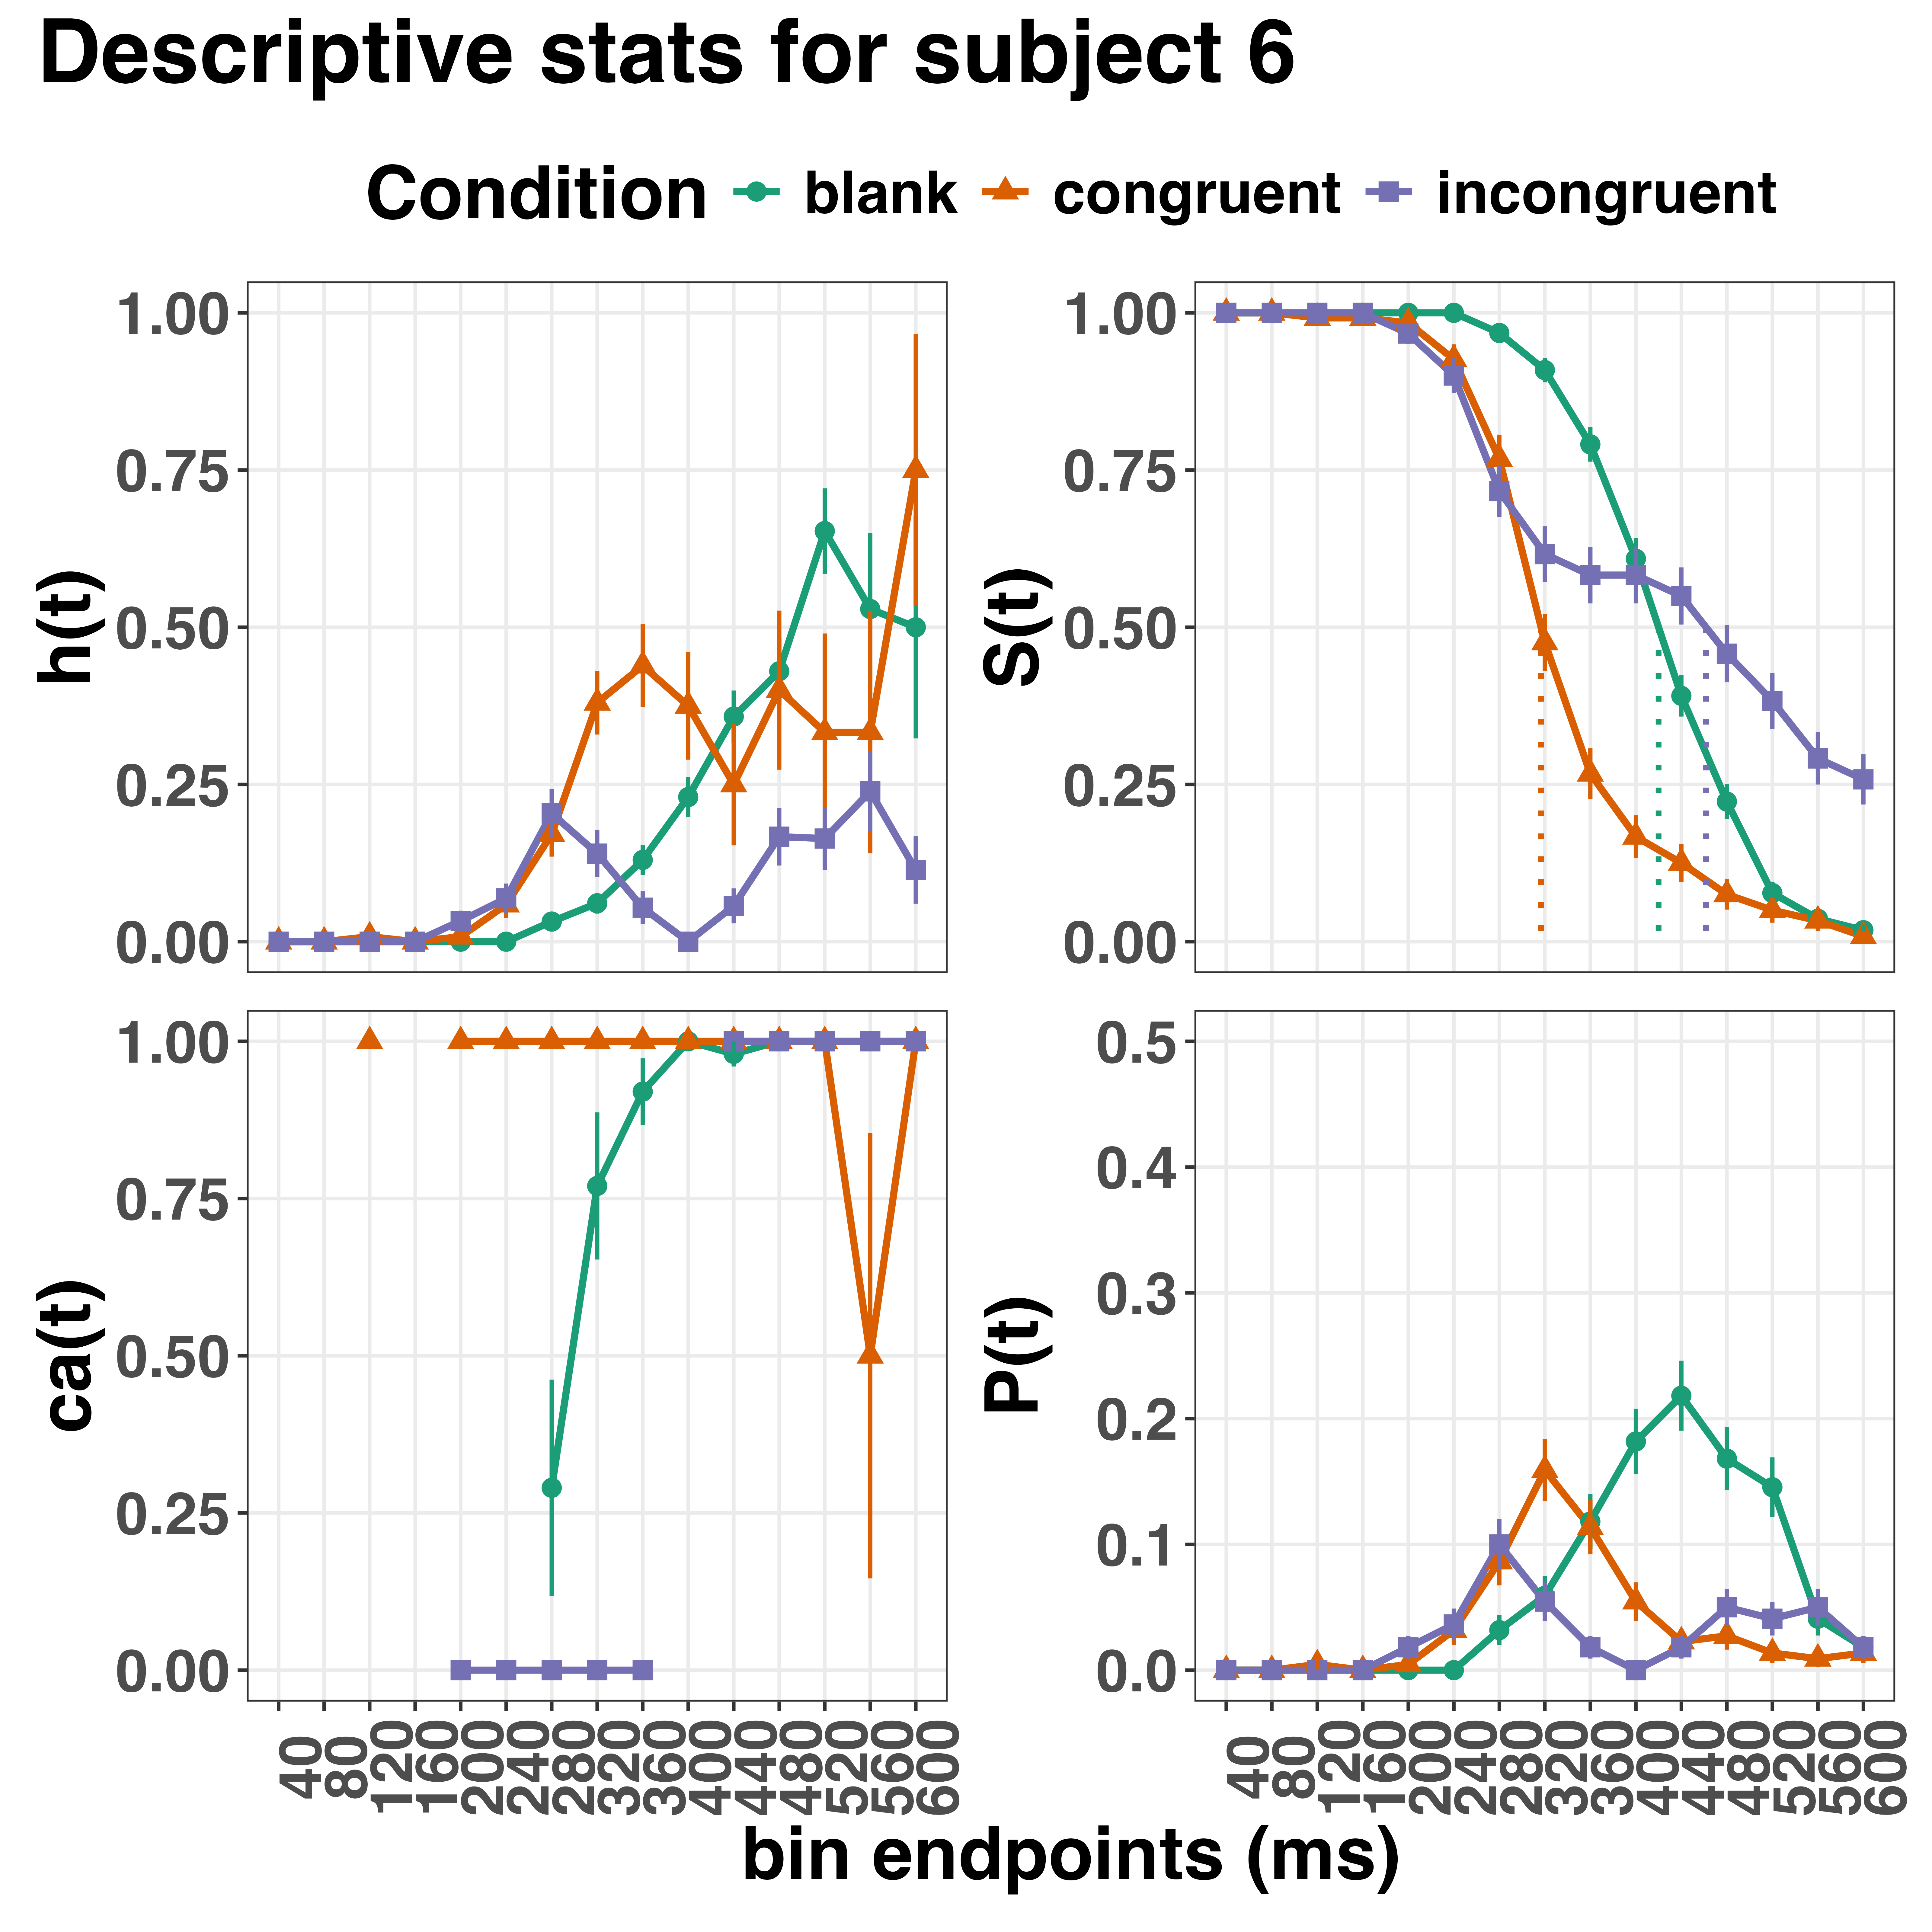
\includegraphics[width=12in,height=0.67\textheight,]{../Tutorial_1_descriptive_stats/figures/Plot_for_subject6_PanisSchmidt} 

}

\caption{Discrete-time hazard, survivor, and conditional accuracy functions for participant 6, as a function of the passage of discrete waiting time.}\label{fig:eha-plot}
\end{figure}

Furthermore, the estimated conditional accuracy values in bin (240,280{]} are 0.29, 1, and 0 for the blank, congruent, and incongruent prime conditions, respectively. In other words, if a response is emitted in bin (240,280{]}, then the probability that it is correct is estimated to be 0.29, 1, and 0 for the blank, congruent, and incongruent prime conditions, respectively.

However, when the waiting time has increased until \emph{400 ms} after target onset, then the conditional probability of response occurrence in the next 40 ms is estimated to be 0.36, 0.25, and 0.07 for the blank, congruent, and incongruent prime conditions, respectively. And when a response does occur in bin (400,440{]}, then the probability that it is correct is estimated to be 0.98, 1, and 1 for the blank, congruent, and incongruent prime conditions, respectively.

These results show that this participant is initially responding to the prime even though (s)he was instructed to only respond to the target, that response competition emerges in the incongruent prime condition around 300 ms, and that only later response are fully controlled by the target stimulus. Qualitatively similar results were obtained for the other five participants. Also, in their second Experiment, Panis and Schmidt (2016) showed that the negative compatibility effect in the mask-present conditions is time-locked to mask onset. This example shows that a simple difference between two means fails to reveal the dynamic behavior people display in many experimental paradigms (Panis, 2020; Panis, Moran, et al., 2020; Panis \& Schmidt, 2022; Panis, Torfs, Gillebert, Wagemans, \& Humphreys, 2017; Panis \& Wagemans, 2009; Schmidt, Panis, Wolkersdorfer, \& Vorberg, 2022). In other words, statistically controlling for the passage of time during data analysis is equally important as experimental control during the design of an experiment, to better understand human behavior in experimental paradigms. As we will show in Tutorials 2 and 3, statistical models for h(t) and ca(t) can each be implemented as generalized linear mixed regression models predicting event occurrence (1/0) and response accuracy (1/0) in each bin of a selected time range, respectively.

\section{Tutorial 2: Fitting Bayesian hazard models}\label{tutorial-2-fitting-bayesian-hazard-models}

\section{Tutorial 3: Fitting Frequentist hazard models}\label{tutorial-3-fitting-frequentist-hazard-models}

\section{Methods}\label{methods}

We report how we determined our sample size, all data exclusions (if any), all manipulations, and all measures in the study.

\subsection{Participants}\label{participants}

\subsection{Material}\label{material}

\subsection{Procedure}\label{procedure}

\subsection{Data analysis}\label{data-analysis}

\section{Results}\label{results}

\section{Discussion}\label{discussion}

\newpage

\section{References}\label{references}

\phantomsection\label{refs}
\begin{CSLReferences}{1}{0}
\bibitem[\citeproctext]{ref-allisonDiscreteTimeMethodsAnalysis1982}
Allison, P. D. (1982). Discrete-{Time Methods} for the {Analysis} of {Event Histories}. \emph{Sociological Methodology}, \emph{13}, 61. \url{https://doi.org/10.2307/270718}

\bibitem[\citeproctext]{ref-allisonSurvivalAnalysisUsing2010}
Allison, P. D. (2010). \emph{Survival analysis using {SAS}: A practical guide} (2. ed). Cary, NC: SAS Press.

\bibitem[\citeproctext]{ref-R-citr}
Aust, F. (2019). \emph{Citr: 'RStudio' add-in to insert markdown citations}. Retrieved from \url{https://github.com/crsh/citr}

\bibitem[\citeproctext]{ref-R-papaja}
Aust, F., \& Barth, M. (2023). \emph{{papaja}: {Prepare} reproducible {APA} journal articles with {R Markdown}}. Retrieved from \url{https://github.com/crsh/papaja}

\bibitem[\citeproctext]{ref-bakerPowerContoursOptimising2021}
Baker, D. H., Vilidaite, G., Lygo, F. A., Smith, A. K., Flack, T. R., Gouws, A. D., \& Andrews, T. J. (2021). Power contours: {Optimising} sample size and precision in experimental psychology and human neuroscience. \emph{Psychological Methods}, \emph{26}(3), 295--314. \url{https://doi.org/10.1037/met0000337}

\bibitem[\citeproctext]{ref-R-tinylabels}
Barth, M. (2023). \emph{{tinylabels}: Lightweight variable labels}. Retrieved from \url{https://cran.r-project.org/package=tinylabels}

\bibitem[\citeproctext]{ref-R-lubridate}
Grolemund, G., \& Wickham, H. (2011). Dates and times made easy with {lubridate}. \emph{Journal of Statistical Software}, \emph{40}(3), 1--25. Retrieved from \url{https://www.jstatsoft.org/v40/i03/}

\bibitem[\citeproctext]{ref-holdenDispersionResponseTimes2009}
Holden, J. G., Van Orden, G. C., \& Turvey, M. T. (2009). Dispersion of response times reveals cognitive dynamics. \emph{Psychological Review}, \emph{116}(2), 318--342. \url{https://doi.org/10.1037/a0014849}

\bibitem[\citeproctext]{ref-kantowitzInterpretationReactionTime2021}
Kantowitz, B. H., \& Pachella, R. G. (2021). The {Interpretation} of {Reaction Time} in {Information-Processing Research} 1. \emph{Human Information Processing}, 41--82. \url{https://doi.org/10.4324/9781003176688-2}

\bibitem[\citeproctext]{ref-kelsoOutlineGeneralTheory2013}
Kelso, J. A. S., Dumas, G., \& Tognoli, E. (2013). Outline of a general theory of behavior and brain coordination. \emph{Neural Networks: The Official Journal of the International Neural Network Society}, \emph{37}, 120--131. \url{https://doi.org/10.1016/j.neunet.2012.09.003}

\bibitem[\citeproctext]{ref-luceResponseTimesTheir1991}
Luce, R. D. (1991). \emph{Response times: Their role in inferring elementary mental organization} (1. issued as paperback). Oxford: Univ. Press.

\bibitem[\citeproctext]{ref-meyerModernMentalChronometry1988}
Meyer, D. E., Osman, A. M., Irwin, D. E., \& Yantis, S. (1988). Modern mental chronometry. \emph{Biological Psychology}, \emph{26}(1-3), 3--67. \url{https://doi.org/10.1016/0301-0511(88)90013-0}

\bibitem[\citeproctext]{ref-R-tibble}
Müller, K., \& Wickham, H. (2023). \emph{Tibble: Simple data frames}. Retrieved from \url{https://CRAN.R-project.org/package=tibble}

\bibitem[\citeproctext]{ref-R-RColorBrewer}
Neuwirth, E. (2022). \emph{RColorBrewer: ColorBrewer palettes}. Retrieved from \url{https://CRAN.R-project.org/package=RColorBrewer}

\bibitem[\citeproctext]{ref-panisHowCanWe2020}
Panis, S. (2020). How can we learn what attention is? {Response} gating via multiple direct routes kept in check by inhibitory control processes. \emph{Open Psychology}, \emph{2}(1), 238--279. \url{https://doi.org/10.1515/psych-2020-0107}

\bibitem[\citeproctext]{ref-panisStudyingDynamicsVisual2020}
Panis, S., Moran, R., Wolkersdorfer, M. P., \& Schmidt, T. (2020). Studying the dynamics of visual search behavior using {RT} hazard and micro-level speed--accuracy tradeoff functions: {A} role for recurrent object recognition and cognitive control processes. \emph{Attention, Perception, \& Psychophysics}, \emph{82}(2), 689--714. \url{https://doi.org/10.3758/s13414-019-01897-z}

\bibitem[\citeproctext]{ref-panisAnalyzingResponseTimes2020}
Panis, S., Schmidt, F., Wolkersdorfer, M. P., \& Schmidt, T. (2020). Analyzing {Response Times} and {Other Types} of {Time-to-Event Data Using Event History Analysis}: {A Tool} for {Mental Chronometry} and {Cognitive Psychophysiology}. \emph{I-Perception}, \emph{11}(6), 2041669520978673. \url{https://doi.org/10.1177/2041669520978673}

\bibitem[\citeproctext]{ref-panisWhatShapingRT2016}
Panis, S., \& Schmidt, T. (2016). What {Is Shaping RT} and {Accuracy Distributions}? {Active} and {Selective Response Inhibition Causes} the {Negative Compatibility Effect}. \emph{Journal of Cognitive Neuroscience}, \emph{28}(11), 1651--1671. \url{https://doi.org/10.1162/jocn_a_00998}

\bibitem[\citeproctext]{ref-panisWhenDoesInhibition2022}
Panis, S., \& Schmidt, T. (2022). When does {``inhibition of return''} occur in spatial cueing tasks? {Temporally} disentangling multiple cue-triggered effects using response history and conditional accuracy analyses. \emph{Open Psychology}, \emph{4}(1), 84--114. \url{https://doi.org/10.1515/psych-2022-0005}

\bibitem[\citeproctext]{ref-panisNeuropsychologicalEvidenceTemporal2017}
Panis, S., Torfs, K., Gillebert, C. R., Wagemans, J., \& Humphreys, G. W. (2017). Neuropsychological evidence for the temporal dynamics of category-specific naming. \emph{Visual Cognition}, \emph{25}(1-3), 79--99. \url{https://doi.org/10.1080/13506285.2017.1330790}

\bibitem[\citeproctext]{ref-panisTimecourseContingenciesPerceptual2009}
Panis, S., \& Wagemans, J. (2009). Time-course contingencies in perceptual organization and identification of fragmented object outlines. \emph{Journal of Experimental Psychology: Human Perception and Performance}, \emph{35}(3), 661--687. \url{https://doi.org/10.1037/a0013547}

\bibitem[\citeproctext]{ref-R-patchwork}
Pedersen, T. L. (2024). \emph{Patchwork: The composer of plots}. Retrieved from \url{https://CRAN.R-project.org/package=patchwork}

\bibitem[\citeproctext]{ref-R-base}
R Core Team. (2024). \emph{R: A language and environment for statistical computing}. Vienna, Austria: R Foundation for Statistical Computing. Retrieved from \url{https://www.R-project.org/}

\bibitem[\citeproctext]{ref-schmidtResponseInhibitionNegative2022}
Schmidt, T., Panis, S., Wolkersdorfer, M. P., \& Vorberg, D. (2022). Response inhibition in the {Negative Compatibility Effect} in the absence of inhibitory stimulus features. \emph{Open Psychology}, \emph{4}(1), 219--230. \url{https://doi.org/10.1515/psych-2022-0012}

\bibitem[\citeproctext]{ref-singerAppliedLongitudinalData2003}
Singer, J. D., \& Willett, J. B. (2003). \emph{Applied longitudinal data analysis: Modeling change and event occurrence}. Oxford ; New York: Oxford University Press.

\bibitem[\citeproctext]{ref-smithSmallBeautifulDefense2018}
Smith, P. L., \& Little, D. R. (2018). Small is beautiful: {In} defense of the small-{N} design. \emph{Psychonomic Bulletin \& Review}, \emph{25}(6), 2083--2101. \url{https://doi.org/10.3758/s13423-018-1451-8}

\bibitem[\citeproctext]{ref-townsendTruthConsequencesOrdinal1990}
Townsend, J. T. (1990). Truth and consequences of ordinal differences in statistical distributions: {Toward} a theory of hierarchical inference. \emph{Psychological Bulletin}, \emph{108}(3), 551--567. \url{https://doi.org/10.1037/0033-2909.108.3.551}

\bibitem[\citeproctext]{ref-wickelgrenSpeedaccuracyTradeoffInformation1977}
Wickelgren, W. A. (1977). Speed-accuracy tradeoff and information processing dynamics. \emph{Acta Psychologica}, \emph{41}(1), 67--85. \url{https://doi.org/10.1016/0001-6918(77)90012-9}

\bibitem[\citeproctext]{ref-R-ggplot2}
Wickham, H. (2016). \emph{ggplot2: Elegant graphics for data analysis}. Springer-Verlag New York. Retrieved from \url{https://ggplot2.tidyverse.org}

\bibitem[\citeproctext]{ref-R-forcats}
Wickham, H. (2023a). \emph{Forcats: Tools for working with categorical variables (factors)}. Retrieved from \url{https://forcats.tidyverse.org/}

\bibitem[\citeproctext]{ref-R-stringr}
Wickham, H. (2023b). \emph{Stringr: Simple, consistent wrappers for common string operations}. Retrieved from \url{https://stringr.tidyverse.org}

\bibitem[\citeproctext]{ref-R-tidyverse}
Wickham, H., Averick, M., Bryan, J., Chang, W., McGowan, L. D., François, R., \ldots{} Yutani, H. (2019). Welcome to the {tidyverse}. \emph{Journal of Open Source Software}, \emph{4}(43), 1686. \url{https://doi.org/10.21105/joss.01686}

\bibitem[\citeproctext]{ref-R-dplyr}
Wickham, H., François, R., Henry, L., Müller, K., \& Vaughan, D. (2023). \emph{Dplyr: A grammar of data manipulation}. Retrieved from \url{https://dplyr.tidyverse.org}

\bibitem[\citeproctext]{ref-R-purrr}
Wickham, H., \& Henry, L. (2023). \emph{Purrr: Functional programming tools}. Retrieved from \url{https://purrr.tidyverse.org/}

\bibitem[\citeproctext]{ref-R-readr}
Wickham, H., Hester, J., \& Bryan, J. (2024). \emph{Readr: Read rectangular text data}. Retrieved from \url{https://readr.tidyverse.org}

\bibitem[\citeproctext]{ref-R-tidyr}
Wickham, H., Vaughan, D., \& Girlich, M. (2024). \emph{Tidyr: Tidy messy data}. Retrieved from \url{https://tidyr.tidyverse.org}

\end{CSLReferences}


\end{document}
